\section{TagModel Class Reference}
\label{classTagModel}\index{TagModel@{TagModel}}
Inheritance diagram for TagModel:\nopagebreak
\begin{figure}[H]
\begin{center}
\leavevmode
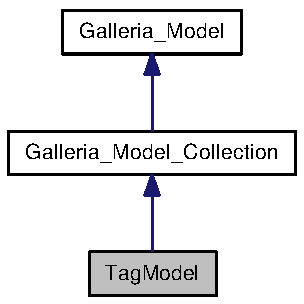
\includegraphics[width=91pt]{classTagModel__inherit__graph}
\end{center}
\end{figure}
Collaboration diagram for TagModel:\nopagebreak
\begin{figure}[H]
\begin{center}
\leavevmode
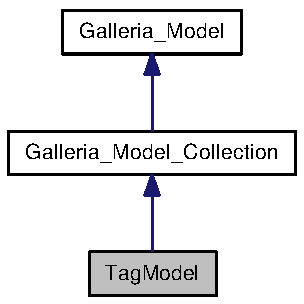
\includegraphics[width=91pt]{classTagModel__coll__graph}
\end{center}
\end{figure}
\subsection*{Public Member Functions}
\begin{CompactItemize}
\item 
{\bf getTagName} (\$tagid)
\item 
{\bf getPics} (\$tagid)
\end{CompactItemize}


\subsection{Detailed Description}


Definition at line 19 of file tagmodel.php.

\subsection{Member Function Documentation}
\index{TagModel@{TagModel}!getTagName@{getTagName}}
\index{getTagName@{getTagName}!TagModel@{TagModel}}
\subsubsection{\setlength{\rightskip}{0pt plus 5cm}TagModel.getTagName (\$ {\em tagid})}\label{classTagModel_33ed8846746b4db91b538171cf6c5669}


Gives name of tag.

This function gets name of specific tag from database.  public \begin{Desc}
\item[Parameters:]
\begin{description}
\item[{\em integer}]\$tagid \end{description}
\end{Desc}
\begin{Desc}
\item[Returns:]string \end{Desc}


Definition at line 30 of file tagmodel.php.

References Galleria\_\-Model.\_\-getConnection().

Here is the call graph for this function:\nopagebreak
\begin{figure}[H]
\begin{center}
\leavevmode

\includegraphics[width=275pt]{classTagModel_33ed8846746b4db91b538171cf6c5669_cgraph}
\end{center}
\end{figure}
\index{TagModel@{TagModel}!getPics@{getPics}}
\index{getPics@{getPics}!TagModel@{TagModel}}
\subsubsection{\setlength{\rightskip}{0pt plus 5cm}TagModel.getPics (\$ {\em tagid})}\label{classTagModel_49a371996b0e0684a5689abd6c160843}


Gives pictures.

This function gets pictures from database according specified tag id.  public \begin{Desc}
\item[Parameters:]
\begin{description}
\item[{\em integer}]\$tagid \end{description}
\end{Desc}
\begin{Desc}
\item[Returns:]array \end{Desc}


Definition at line 46 of file tagmodel.php.

References Galleria\_\-Model.\_\-fetchObjects(), Galleria\_\-Model.\_\-getConnection(), Galleria\_\-Model.\_\-prepareIn(), Galleria\_\-Auth.getObject(), and Galleria\_\-Auth.isLogged().

Here is the call graph for this function:\nopagebreak
\begin{figure}[H]
\begin{center}
\leavevmode
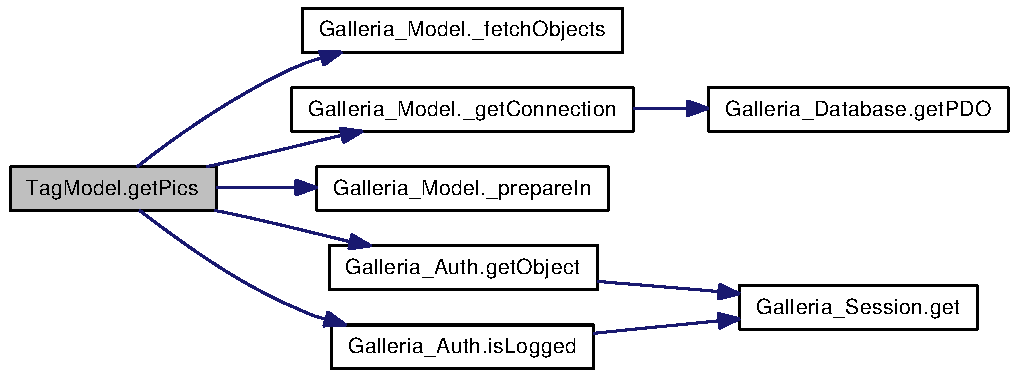
\includegraphics[width=262pt]{classTagModel_49a371996b0e0684a5689abd6c160843_cgraph}
\end{center}
\end{figure}


The documentation for this class was generated from the following file:\begin{CompactItemize}
\item 
/var/www/galleria/data/site/mvc/model/{\bf tagmodel.php}\end{CompactItemize}
